\chapter*{Supplementary}
\addcontentsline{toc}{chapter}{Supplementary}

\begin{figure}[h!]
  \centering
  \begin{subfigure}[b]{\textwidth}
    \centering
    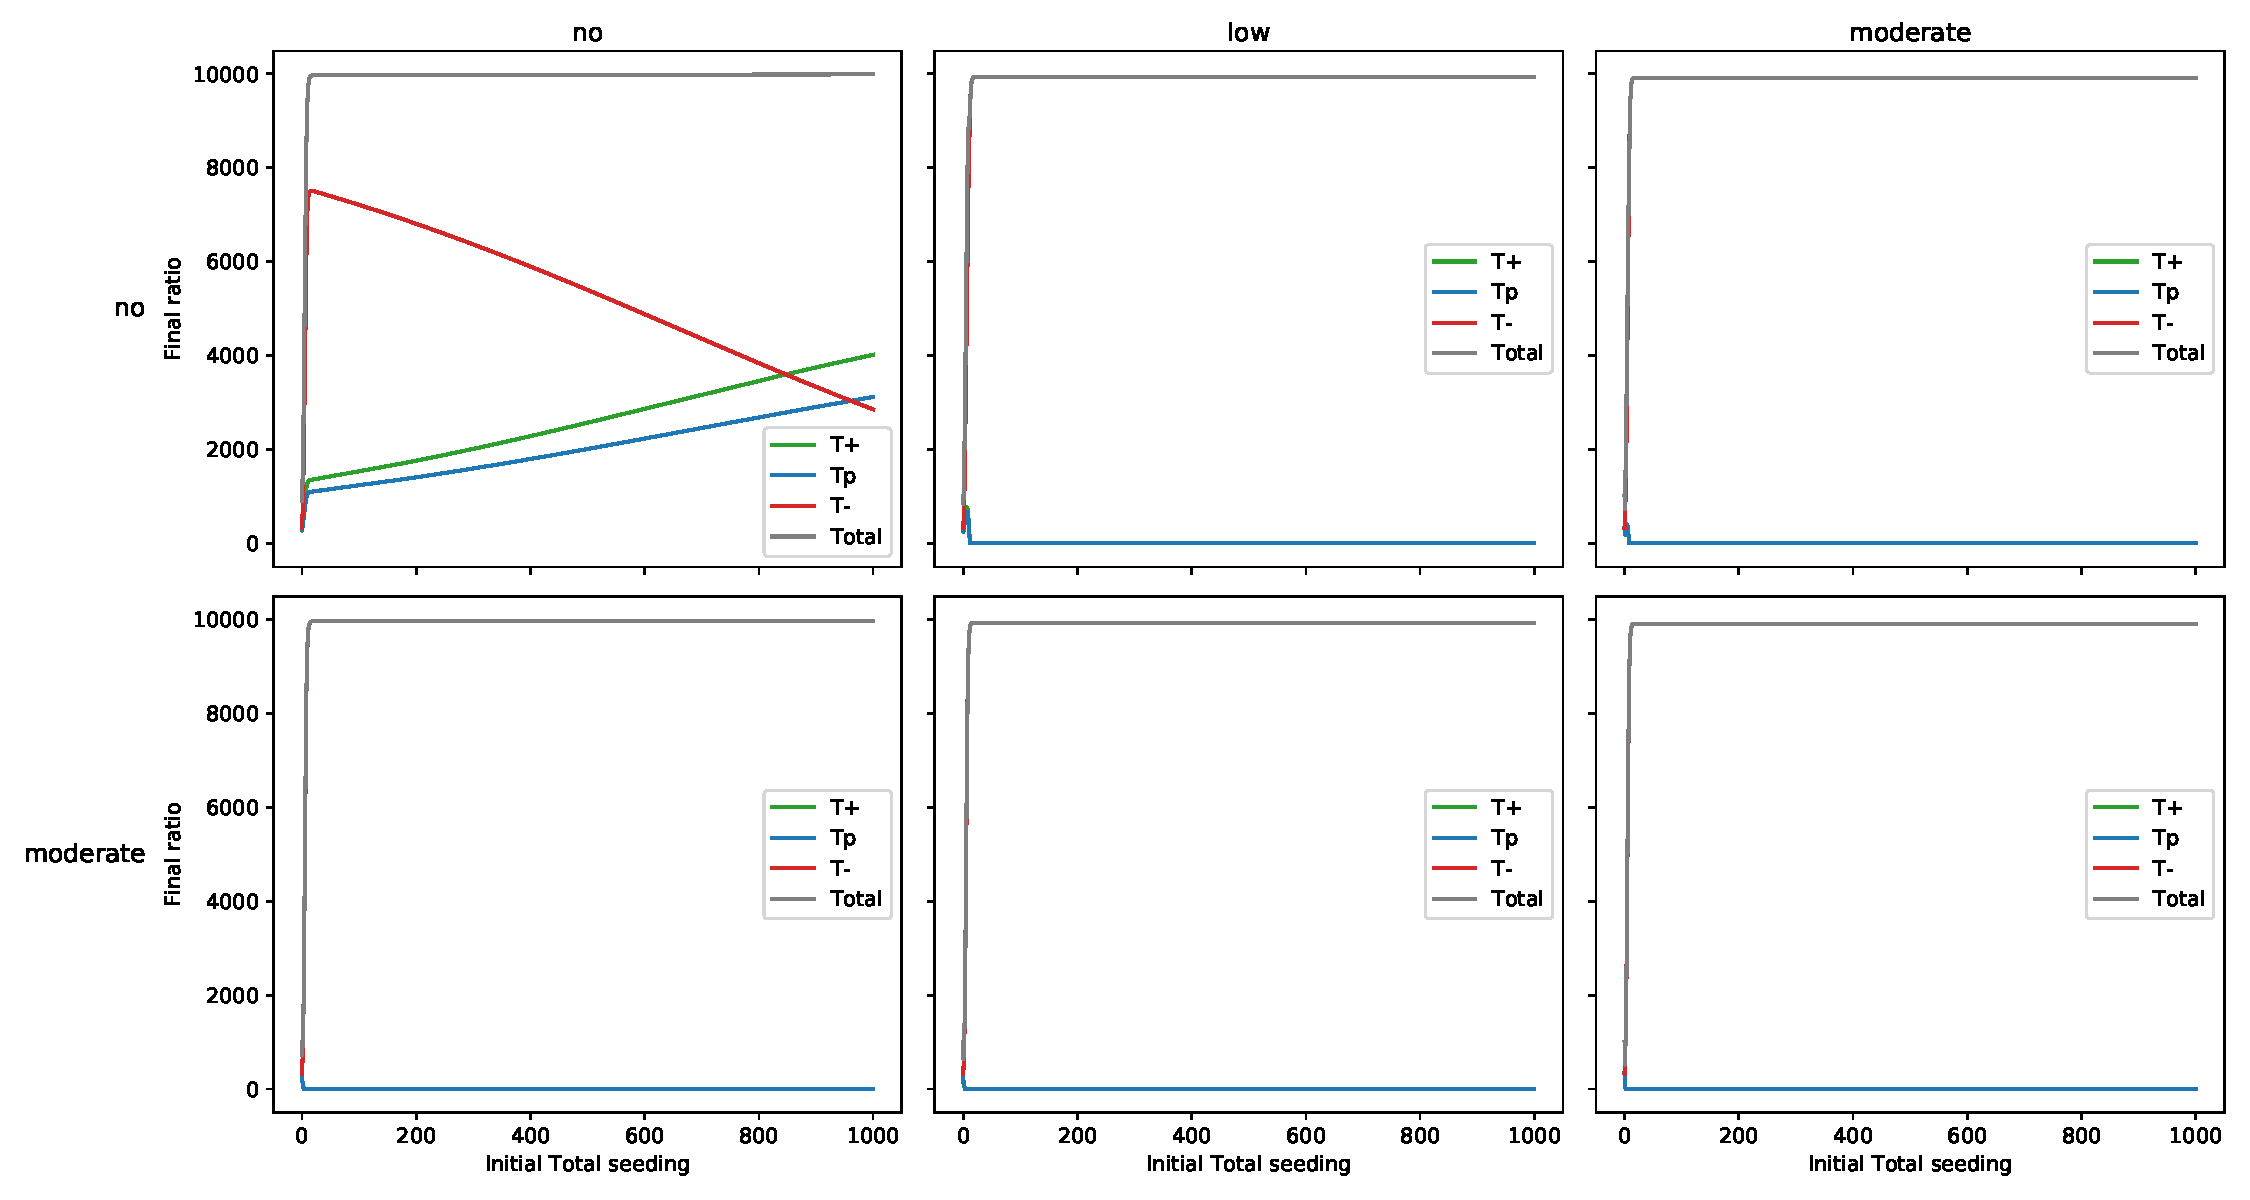
\includegraphics[width=\textwidth]{All3_efficiency_1:1:1-1000}
    \caption{Equal Seeding - $T^p:T^+:T^-$ :: 1:1:1, Initial Total seeding: 1000}
    \label{fig_all3-time-series_1:1:1-1000}
  \end{subfigure}
\end{figure}
\begin{figure}[h!]\ContinuedFloat
  \centering
  \begin{subfigure}[b]{\textwidth}
    \centering
    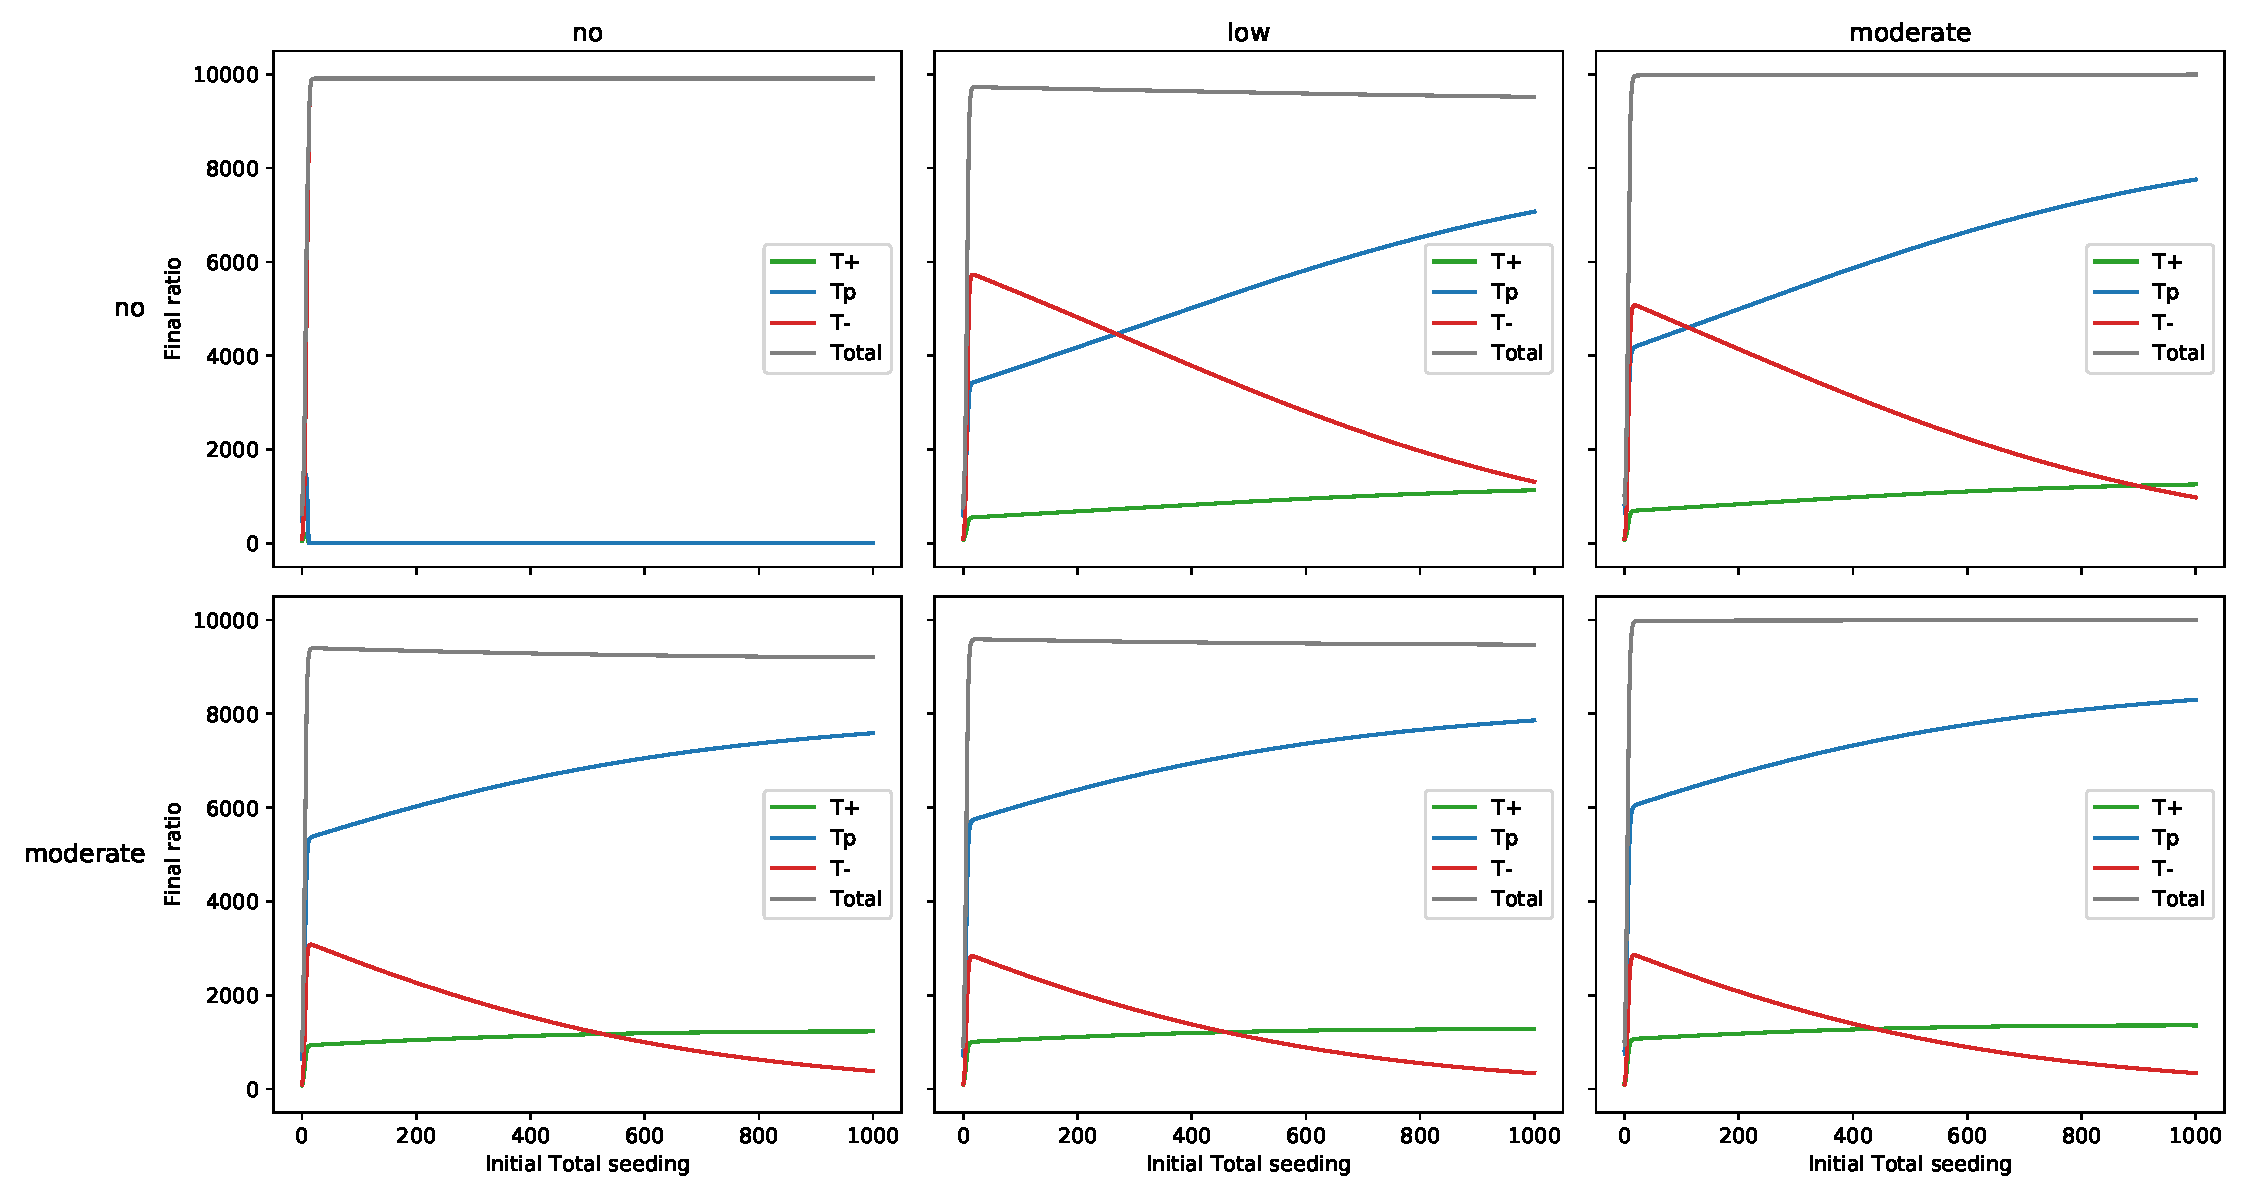
\includegraphics[width=\textwidth]{All3_efficiency_8:1:1-1000}
    \caption{High $T^p$ seeding- $T^p:T^+:T^-$ :: 8:1:1, Initial Total seeding: 1000}
    \label{fig_all3-time-series_8:1:1-1000}
  \end{subfigure}
  \begin{subfigure}[b]{\textwidth}
    \centering
    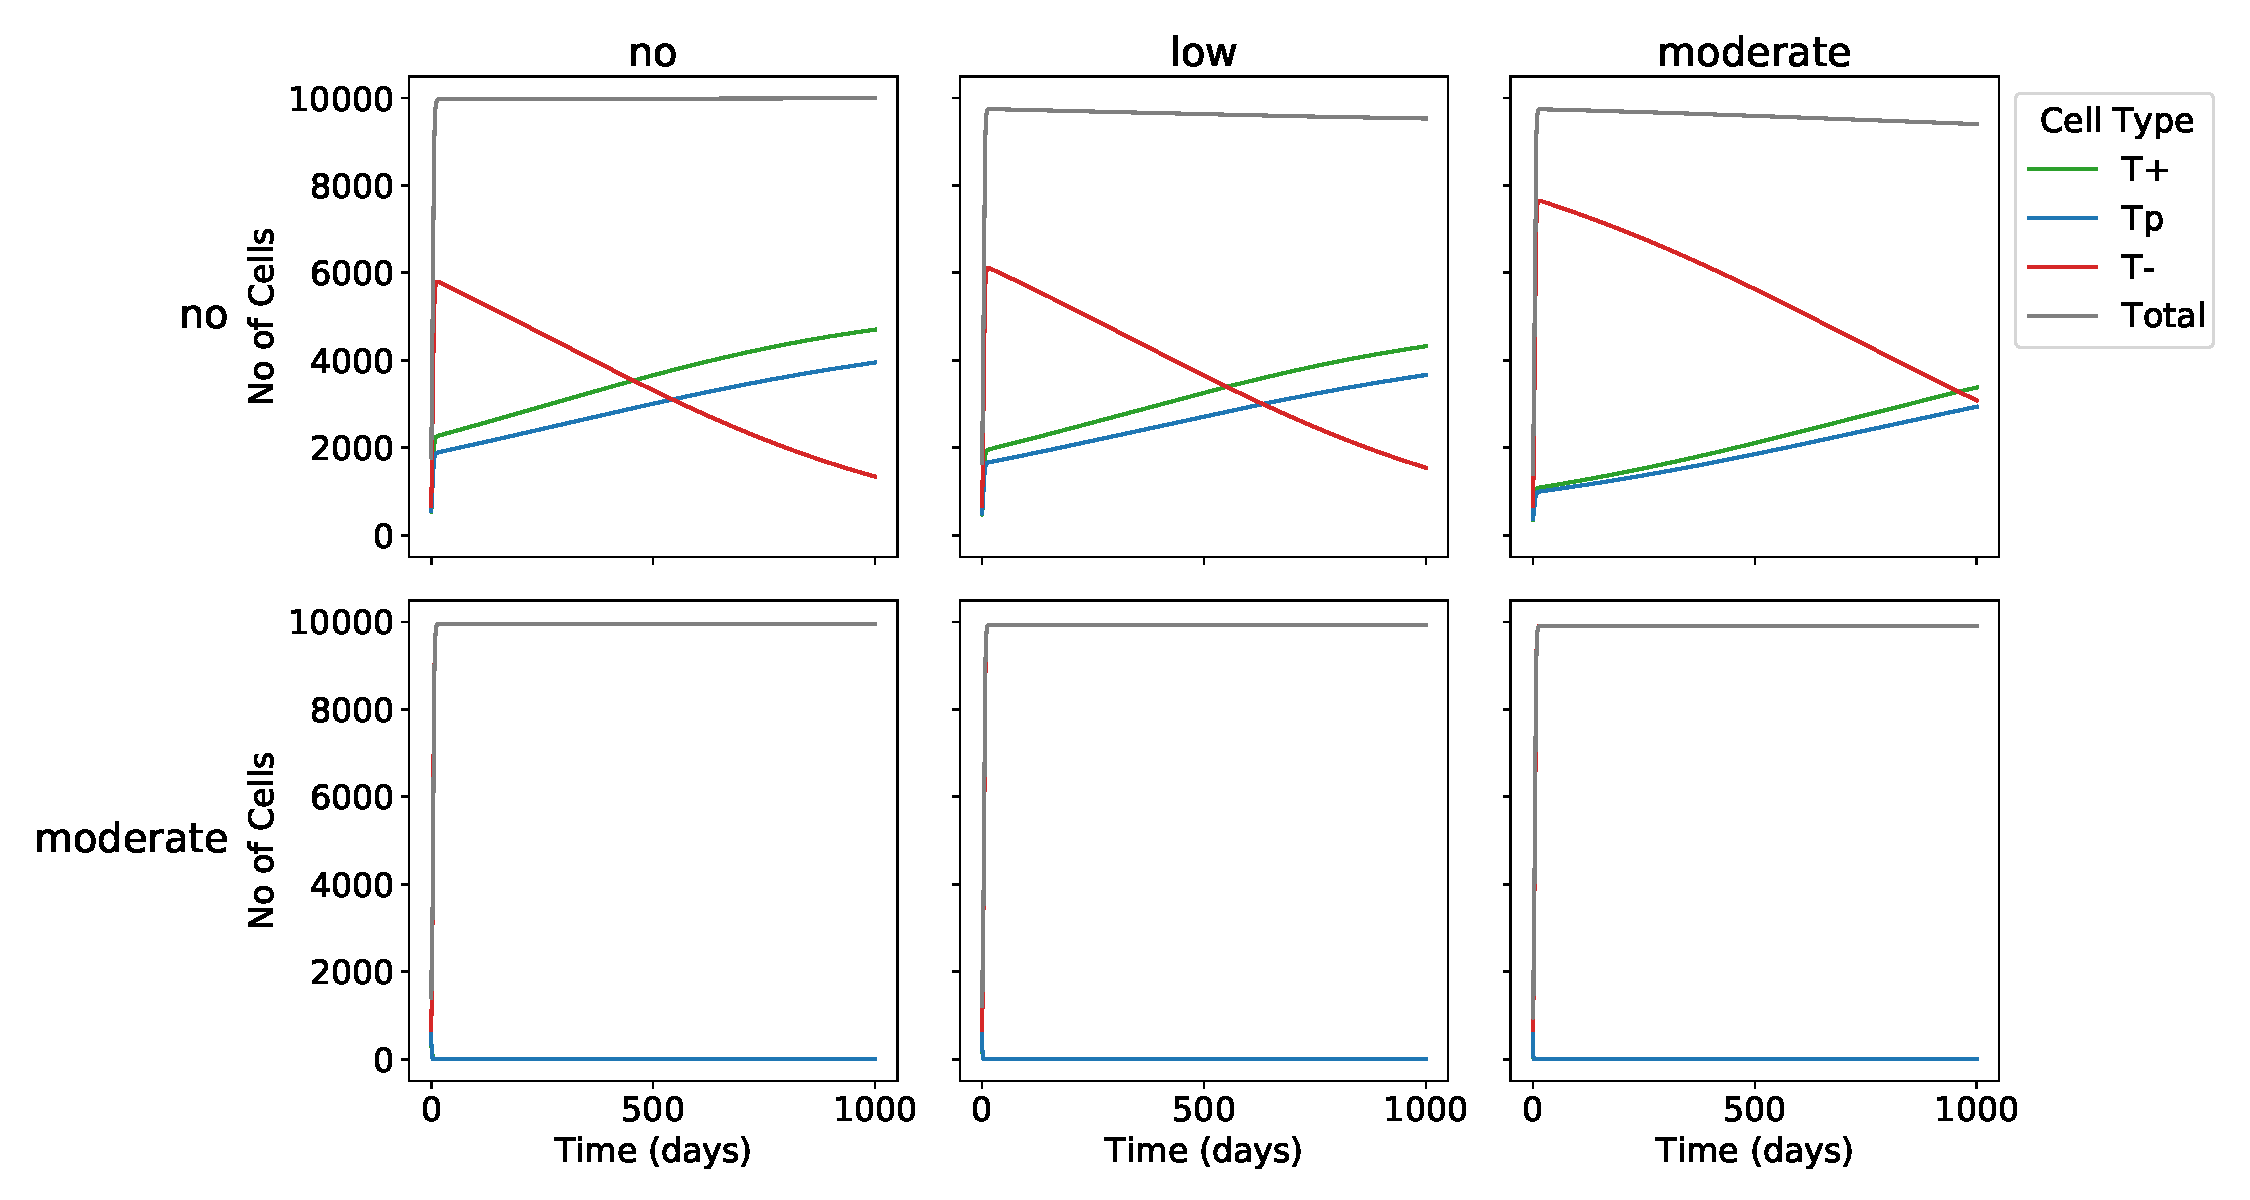
\includegraphics[width=\textwidth]{All3_efficiency_1:1:1-2000}
    \caption{Equal Seeding - $T^p:T^+:T^-$ :: 1:1:1, Initial Total seeding: 2000}
    \label{fig_all3-time-series_1:1:1-2000}
  \end{subfigure}
\end{figure}
\begin{figure}[h!]\ContinuedFloat
  \centering
  \begin{subfigure}[b]{\textwidth}
    \centering
    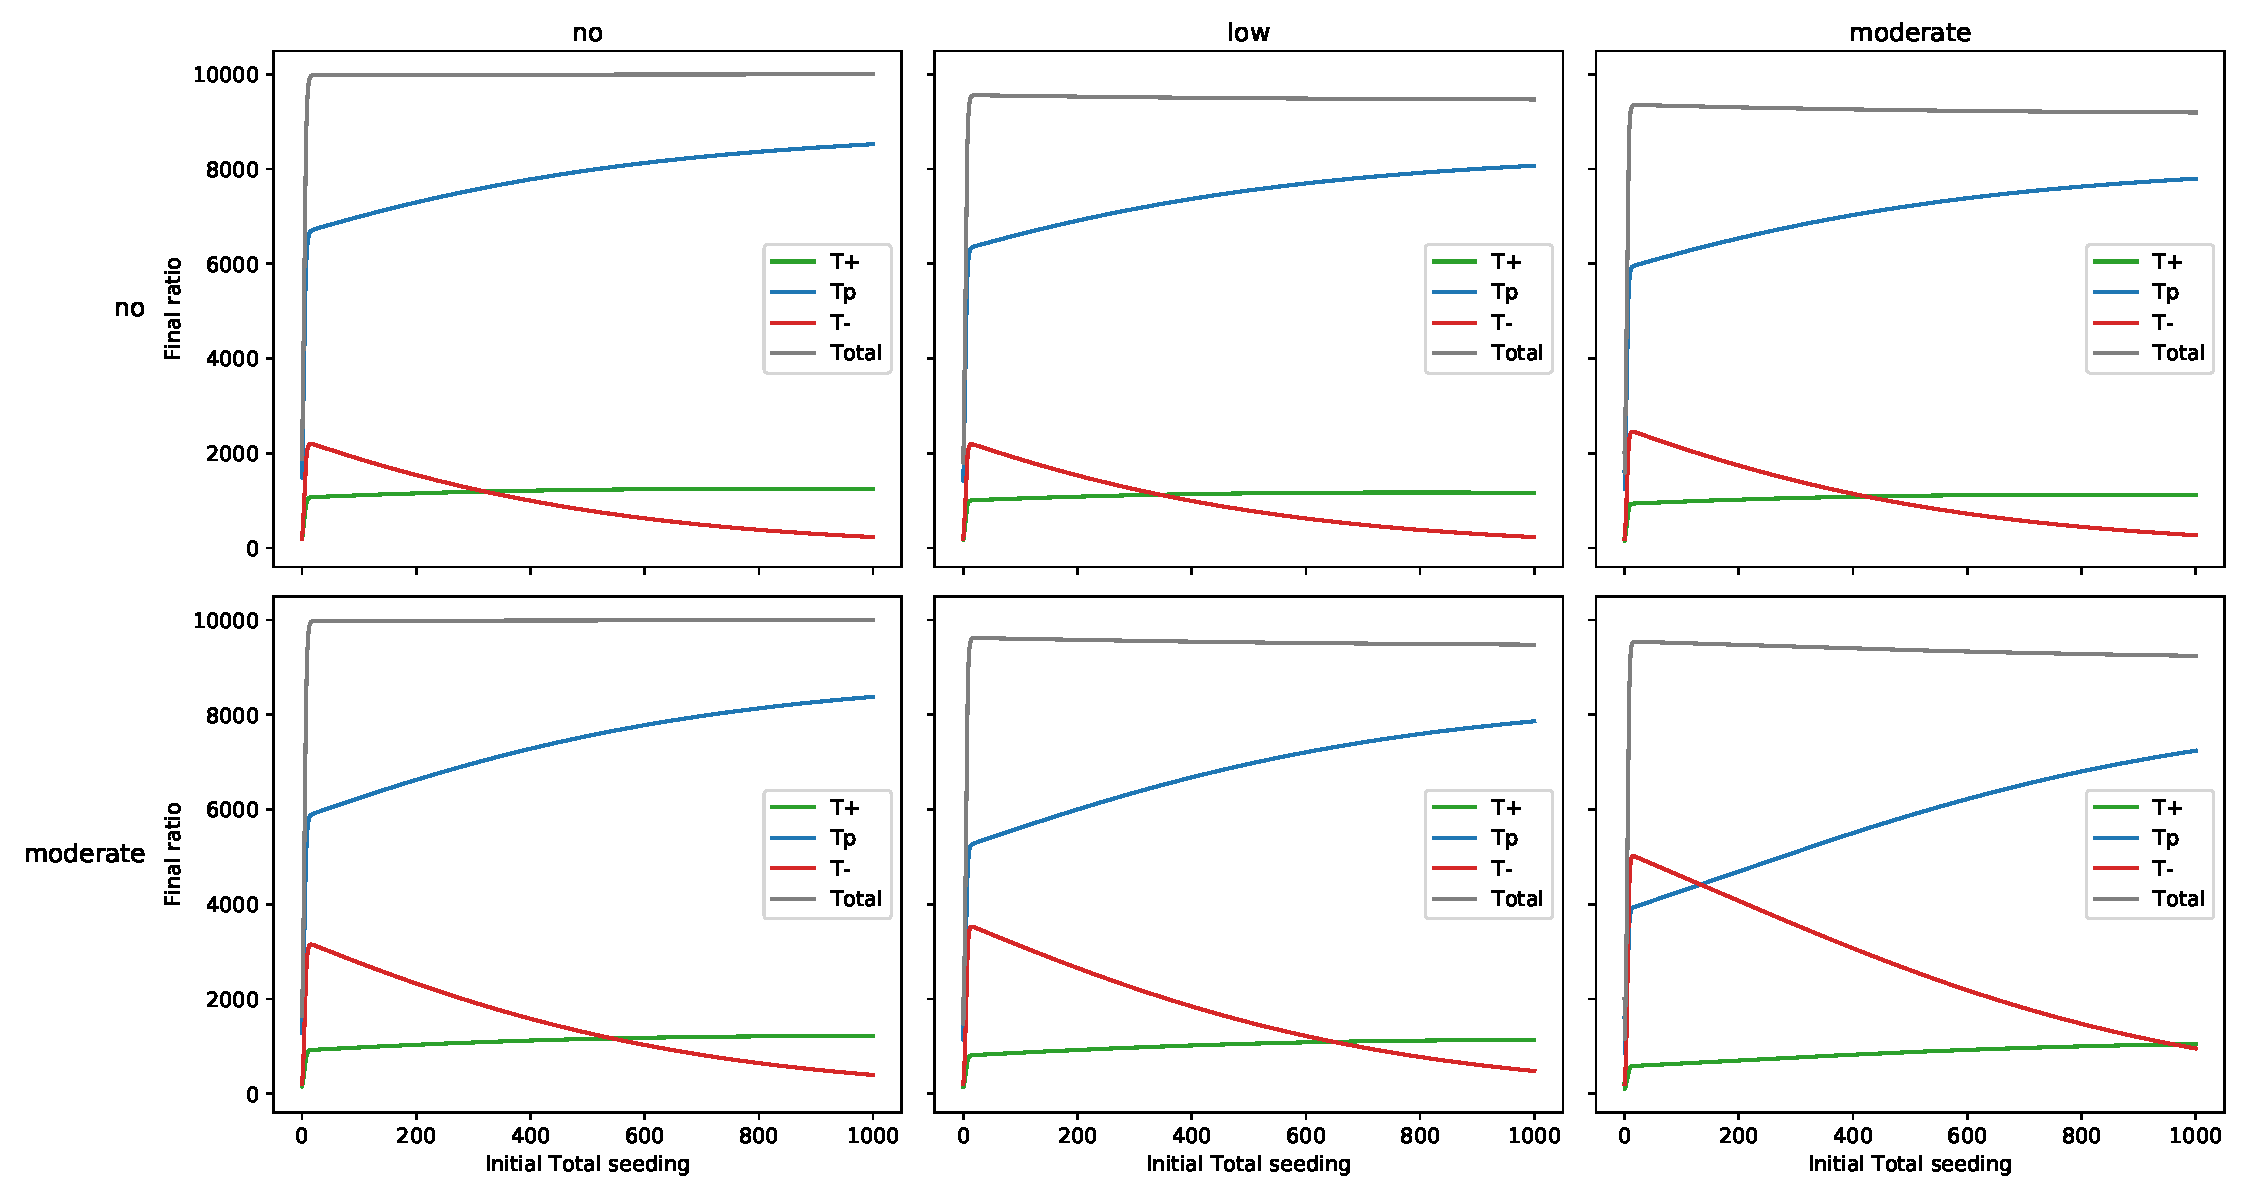
\includegraphics[width=\textwidth]{All3_efficiency_8:1:1-2000}
    \caption{High $T^p$ seeding- $T^p:T^+:T^-$ :: 8:1:1, Initial Total seeding: 2000}
    \label{fig_all3-time-series_8:1:1-2000}
  \end{subfigure}
  \begin{subfigure}[b]{\textwidth}
    \centering
    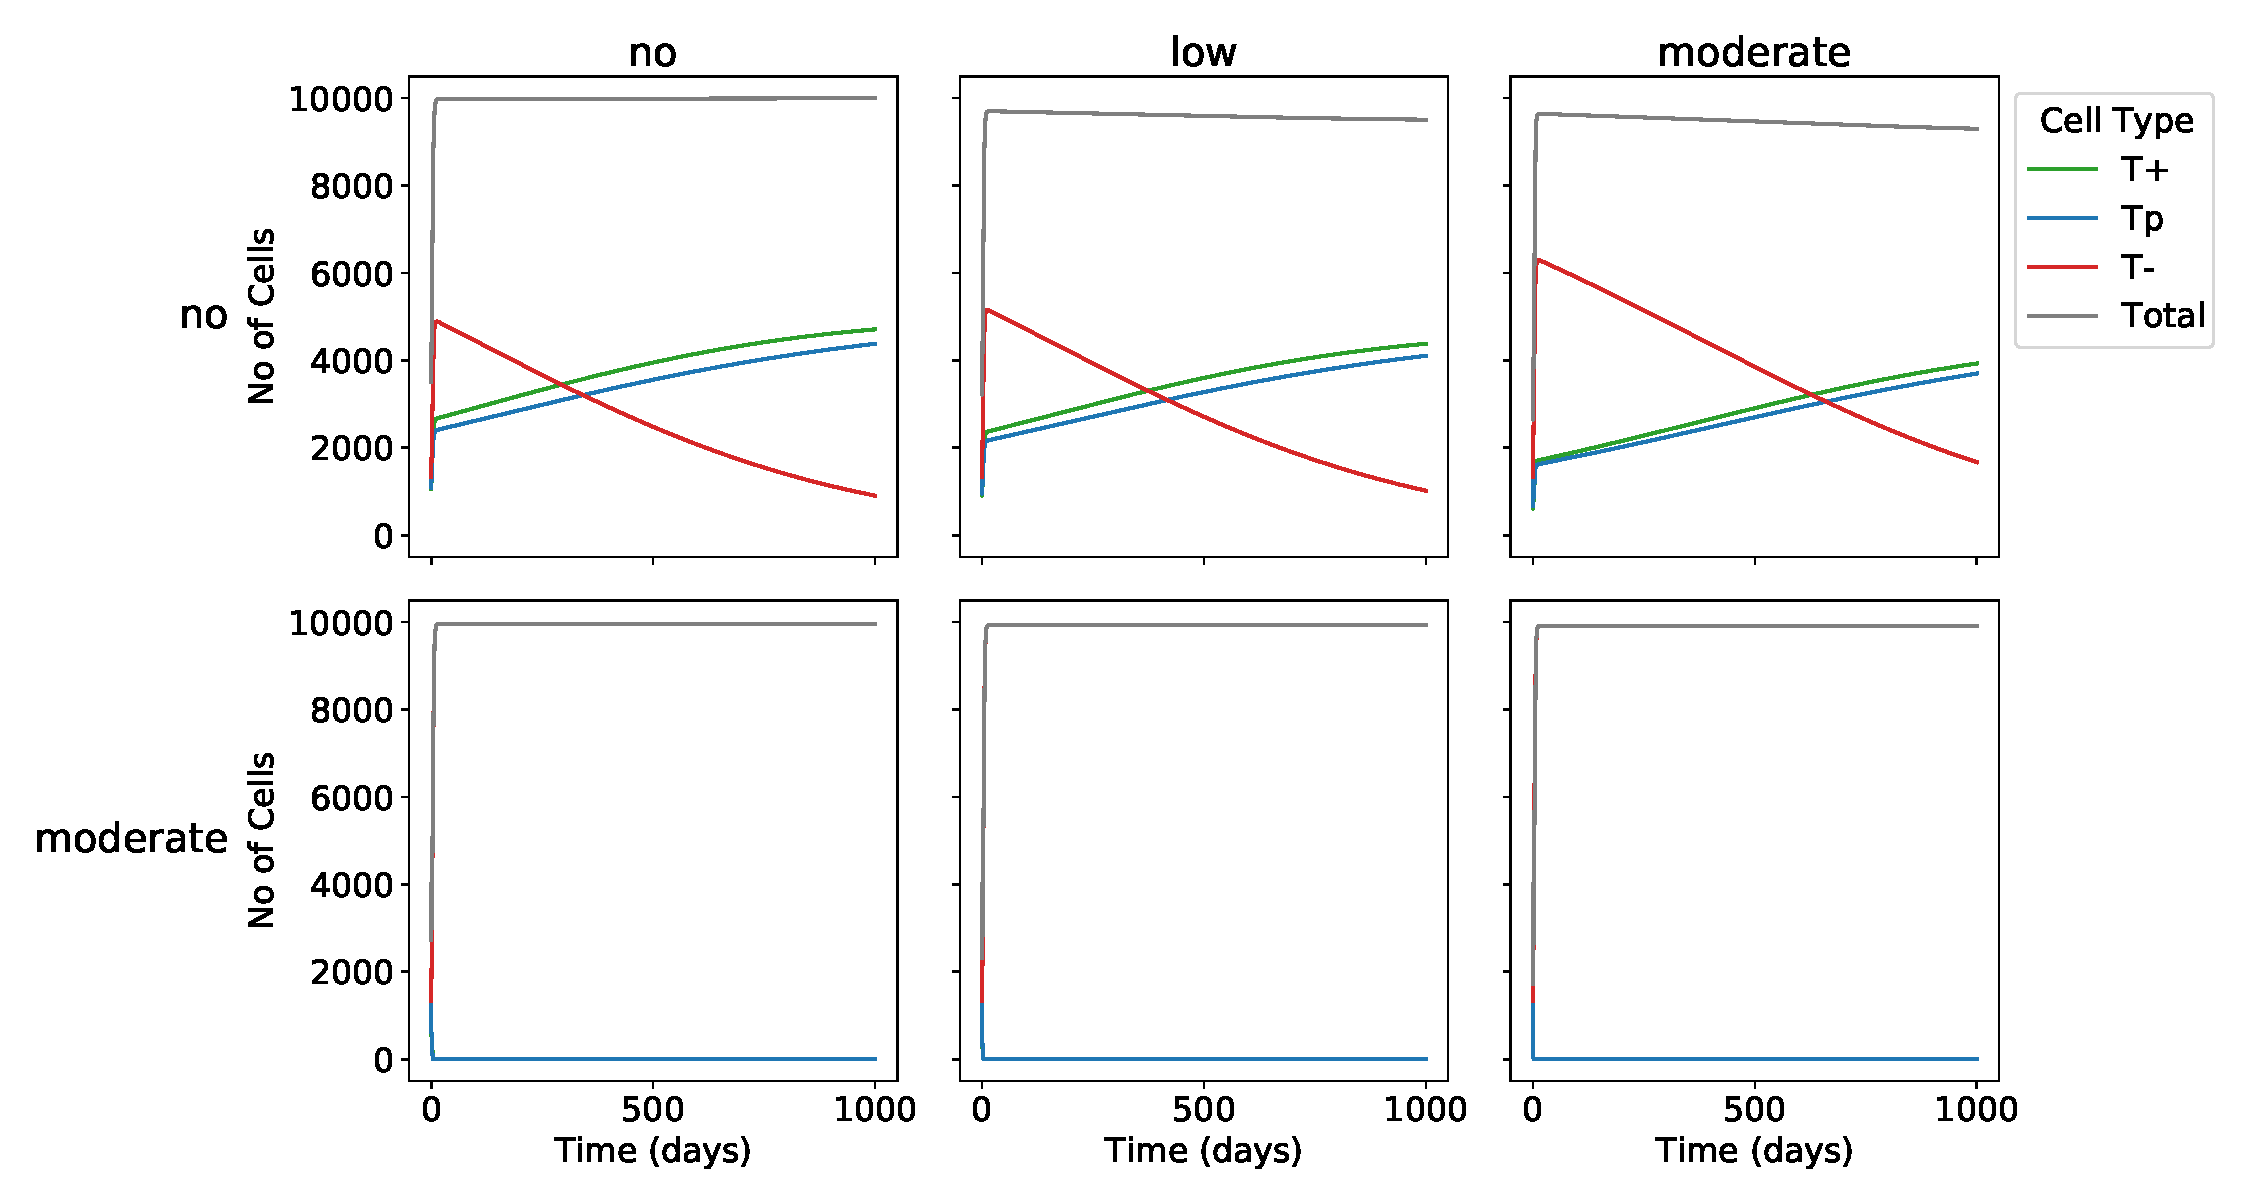
\includegraphics[width=\textwidth]{All3_efficiency_1:1:1-4000}
    \caption{Equal Seeding - $T^p:T^+:T^-$ :: 1:1:1, Initial Total seeding: 4000}
    \label{fig_all3-time-series_1:1:1-4000}
  \end{subfigure}
\end{figure}
\begin{figure}[h!]\ContinuedFloat
  \centering
  \begin{subfigure}[b]{\textwidth}
    \centering
    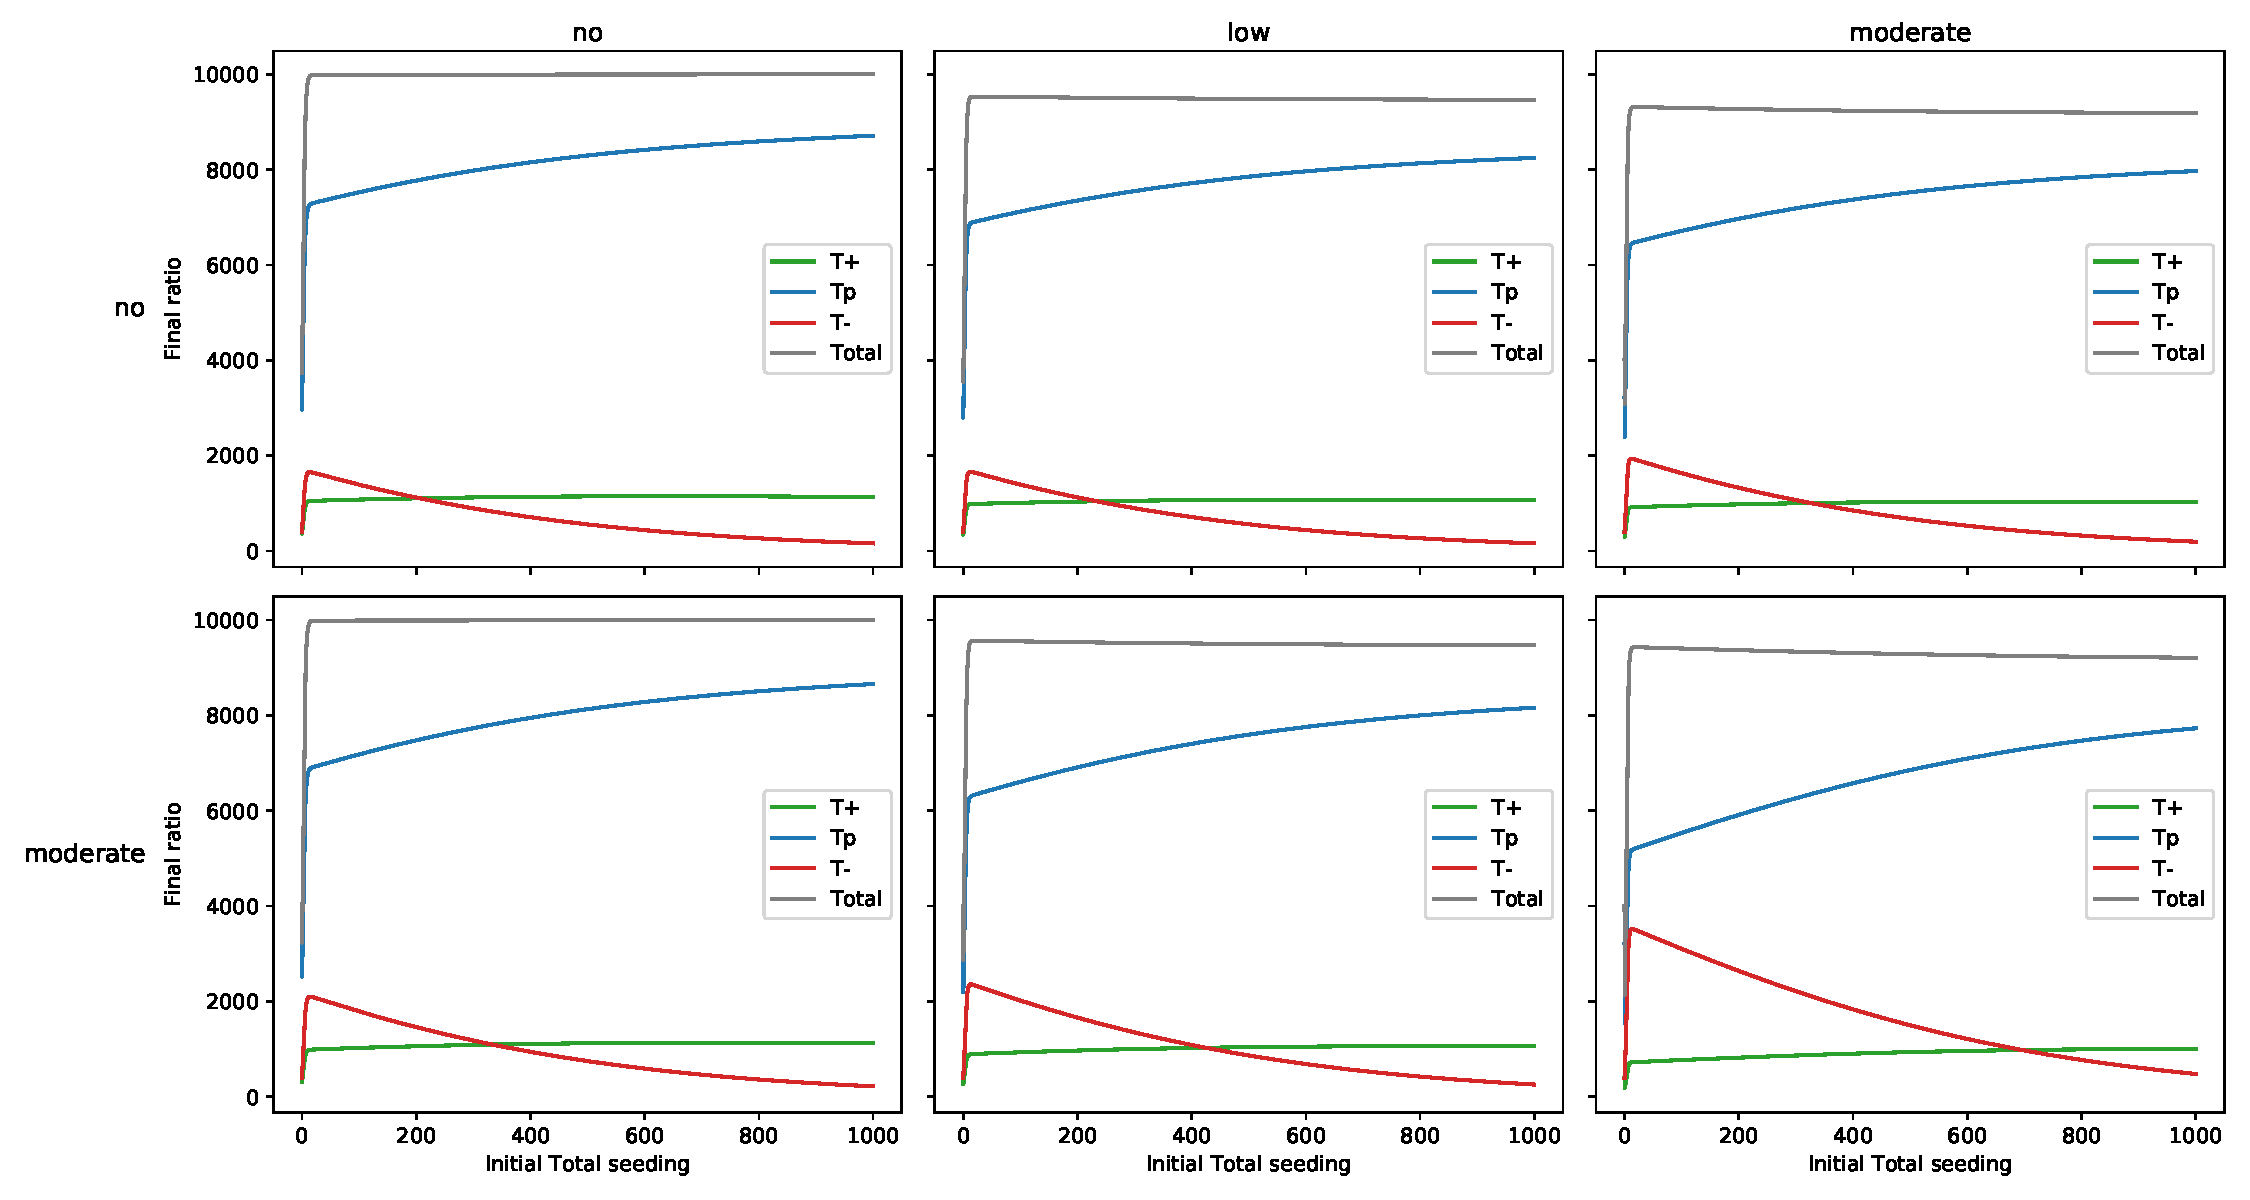
\includegraphics[width=\textwidth]{All3_efficiency_8:1:1-4000}
    \caption{High $T^p$ seeding- $T^p:T^+:T^-$ :: 8:1:1, Initial Total seeding: 4000}
    \label{fig_all3-time-series_8:1:1-4000}
  \end{subfigure}
  \caption[Timeseries of all 3 cell types under different limitations]{Timeseries of all 3 cell types under different oxygen limitation (columns), testosterone limitation (rows) and initial seeding proportions, initial total seeding (subfigures).}
  \label{fig_all3-time-series}
\end{figure}

\begin{figure}[h!]
  \centering
  \begin{subfigure}[b]{\textwidth}
    \centering
    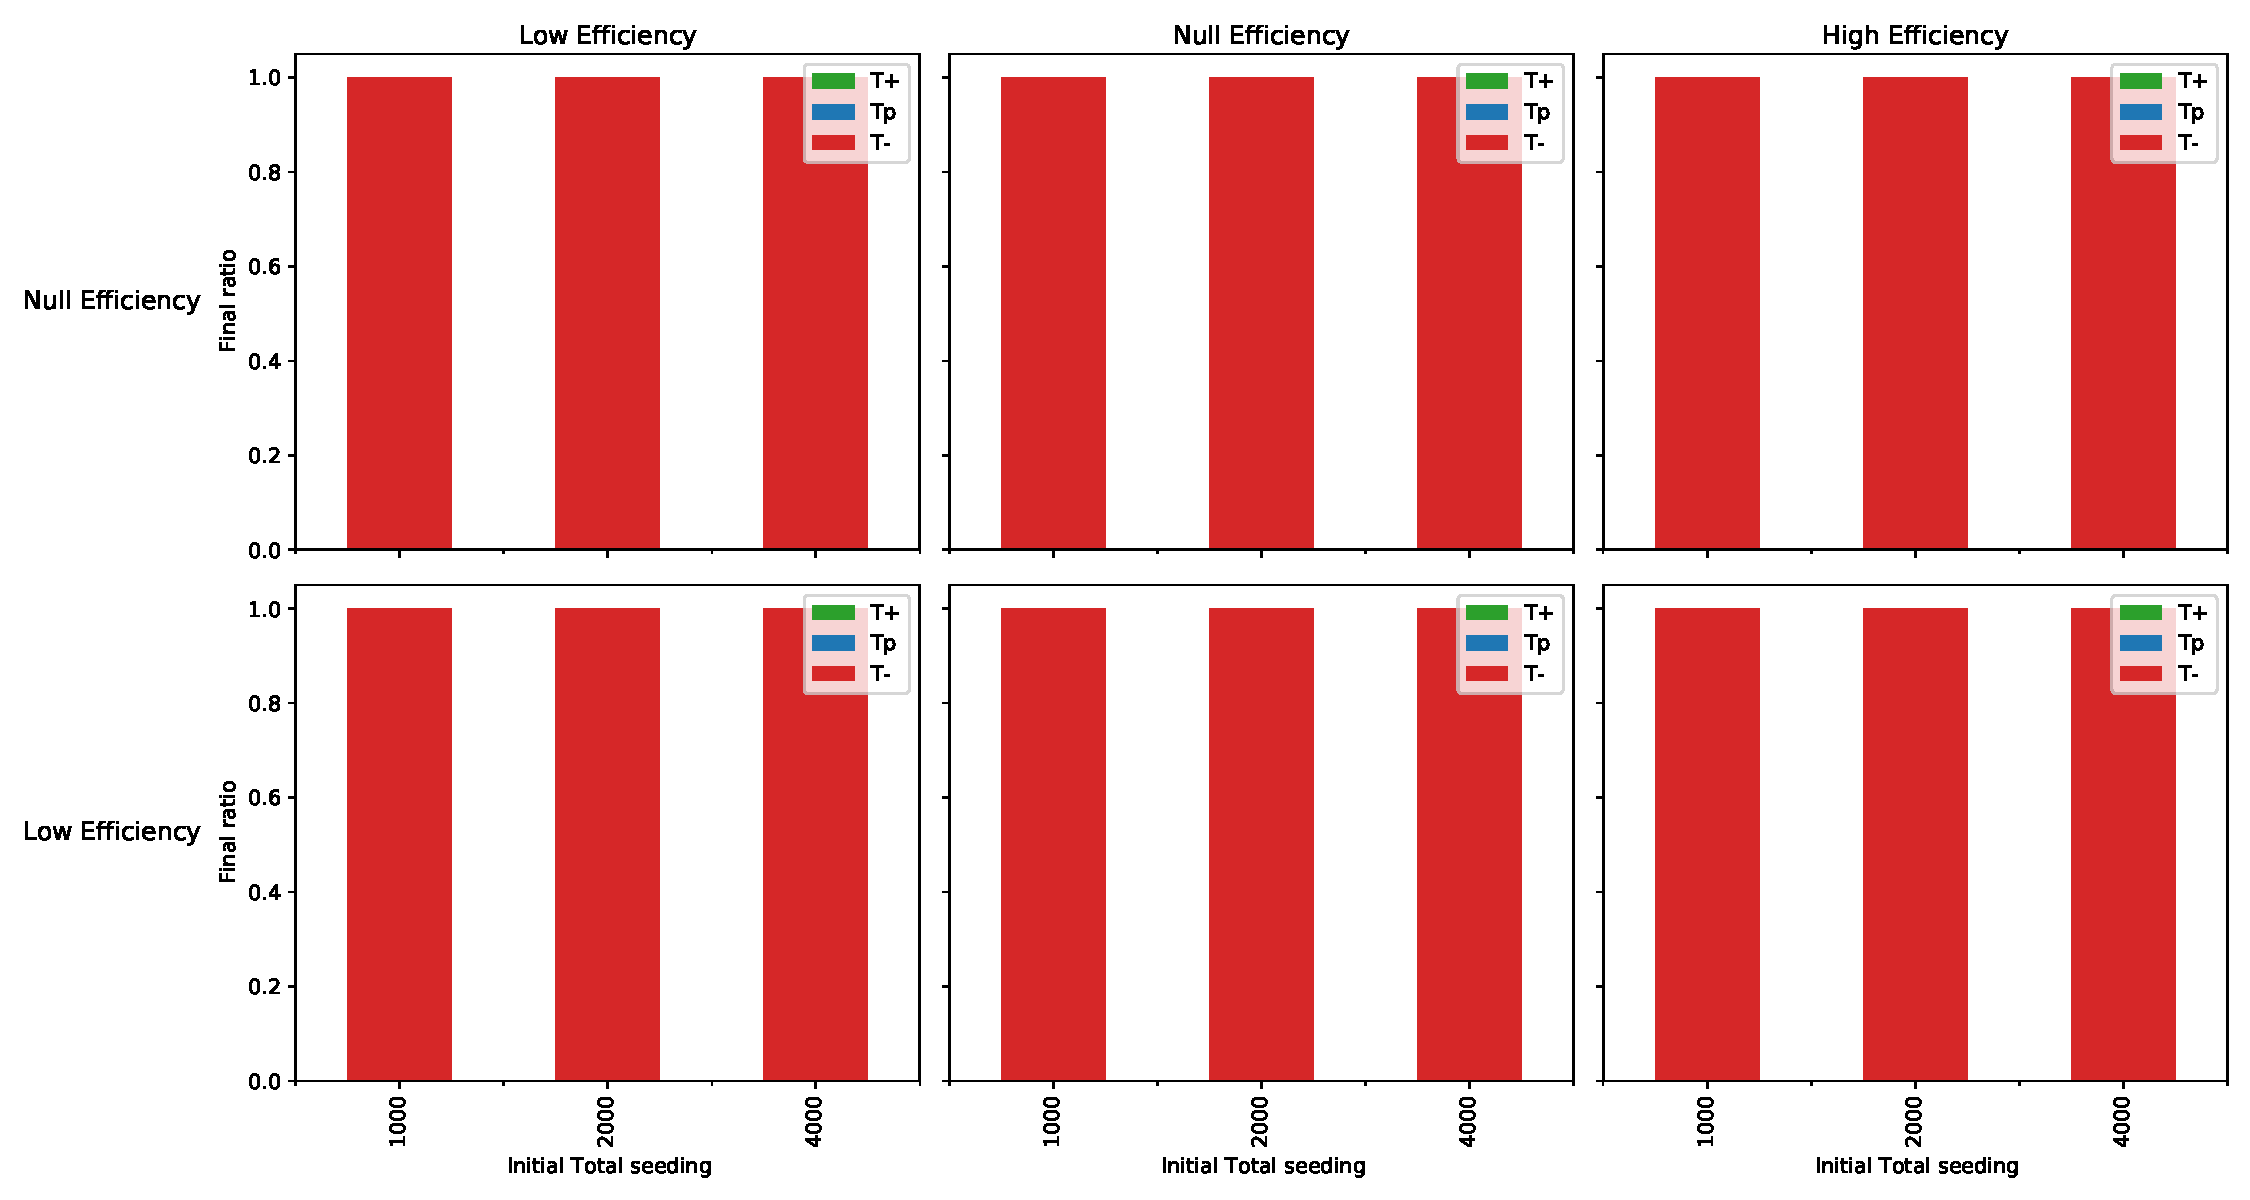
\includegraphics[width=0.9\textwidth]{All3_efficiency-mixed_1:1:1}
    \caption{Equal Seeding - $T^p:T^+:T^-$ :: 1:1:1 }
    \label{fig_all3-mixed_1:1:1}
  \end{subfigure}
  \begin{subfigure}[b]{\textwidth}
    \centering
    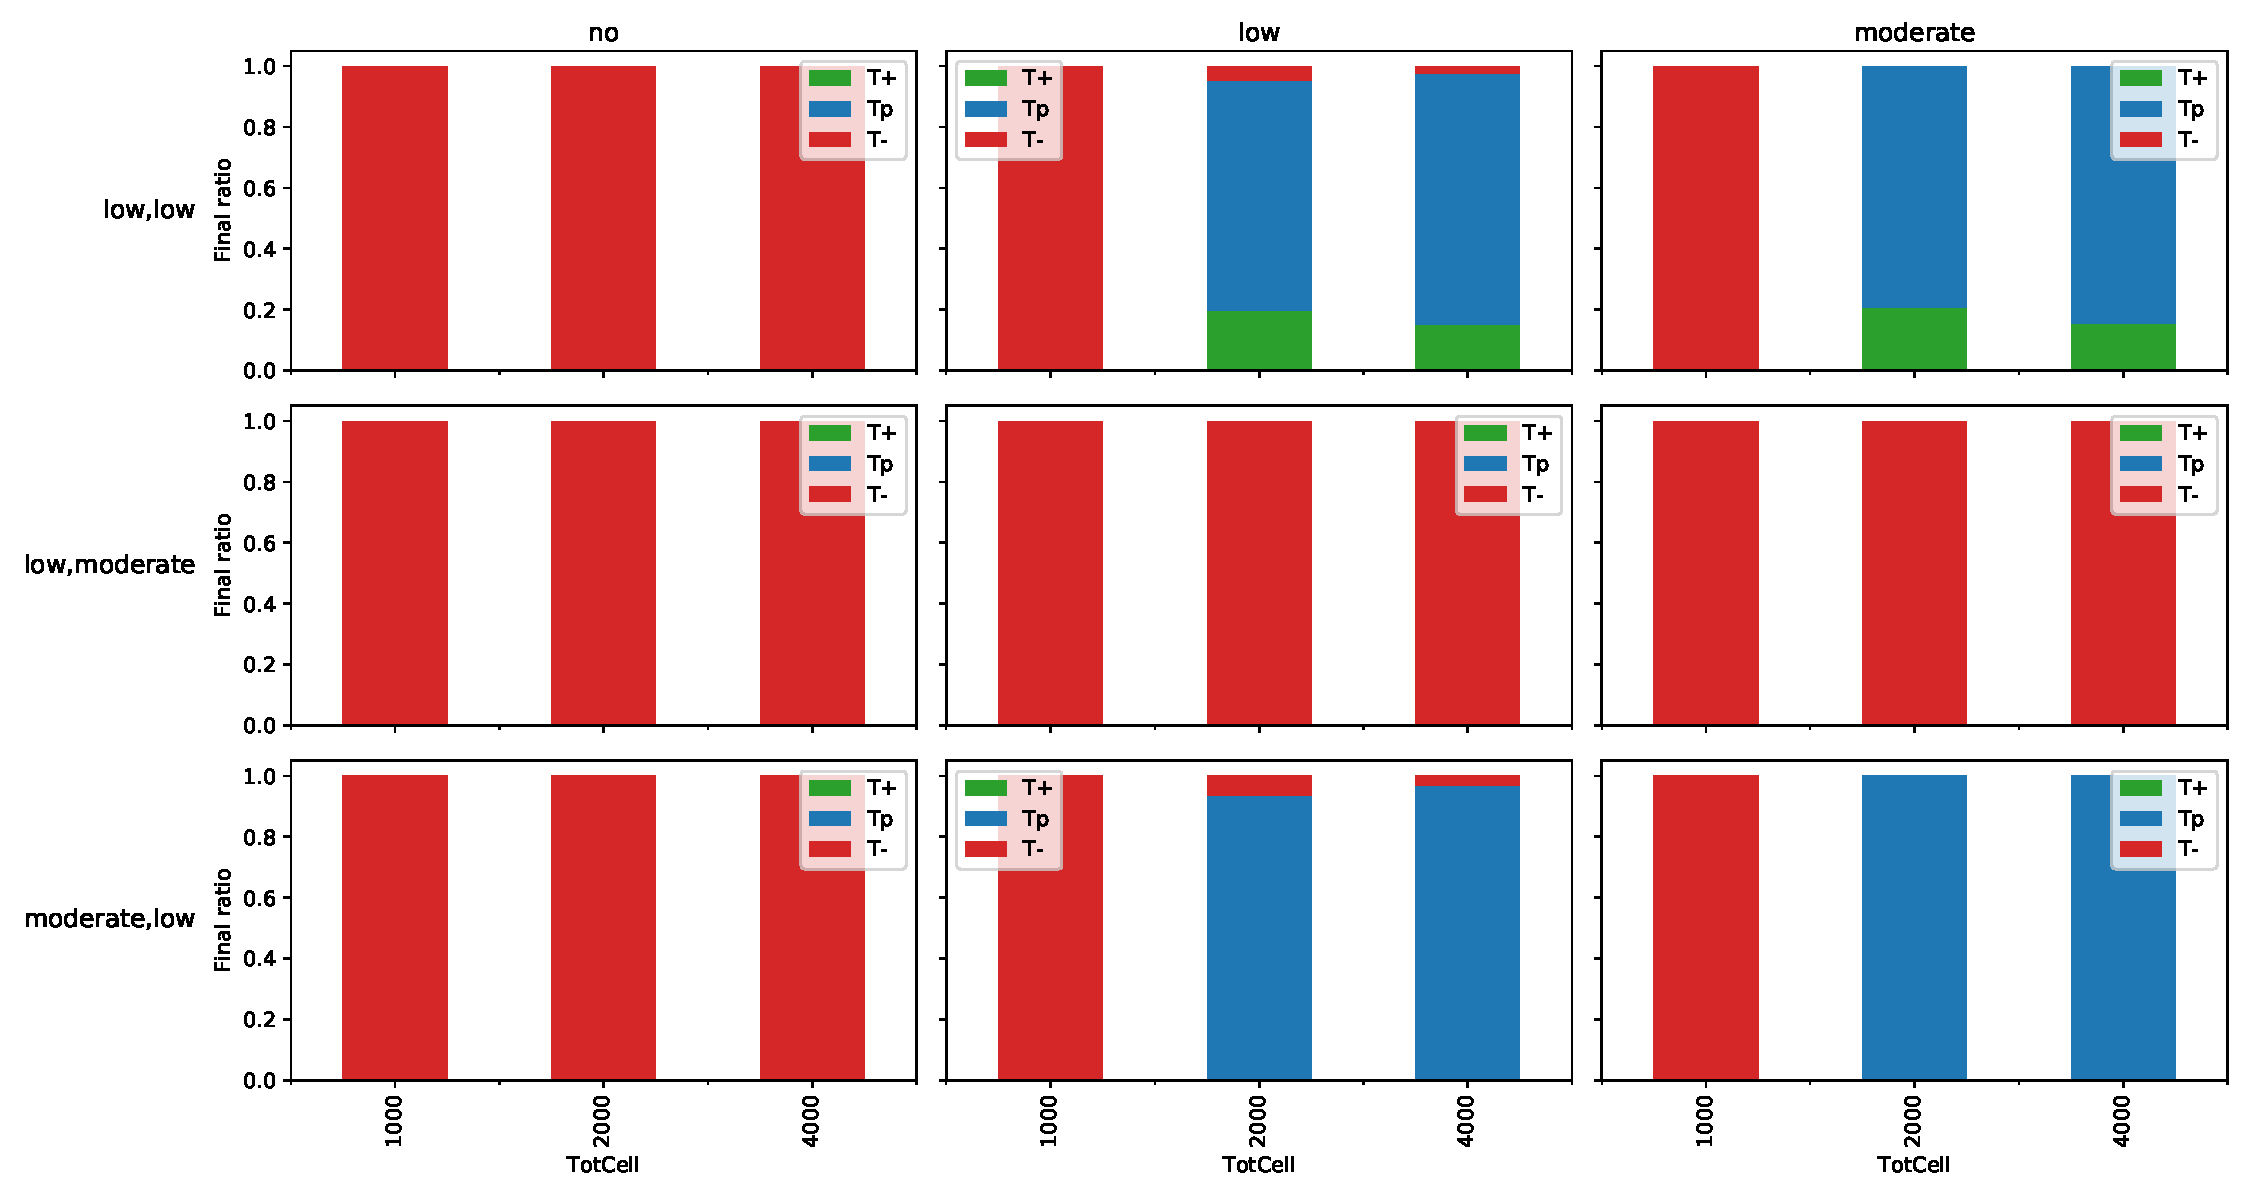
\includegraphics[width=0.9\textwidth]{All3_efficiency-mixed_8:1:1}
    \caption{High $T^p$ seeding- 8:1:1 :: $T^p:T^+:T^-$}
    \label{fig_all3-mixed_8:1:1}
  \end{subfigure}
  \caption[Final ratio of all 3 cell types runs under different limitations for each cell type]{Final ratio of all 3 cell types runs under different oxygen limitations of $T^-$ (columns), oxygen efficiencies of $T^+$, $T^p$ (rows) and initial seeding proportions (subfigures). $T^p$ has low testosterone efficiency.}
  \label{fig_all3-mixed}
\end{figure}

\begin{figure}[h!]
  \centering
  \begin{subfigure}[b]{\textwidth}
    \centering
    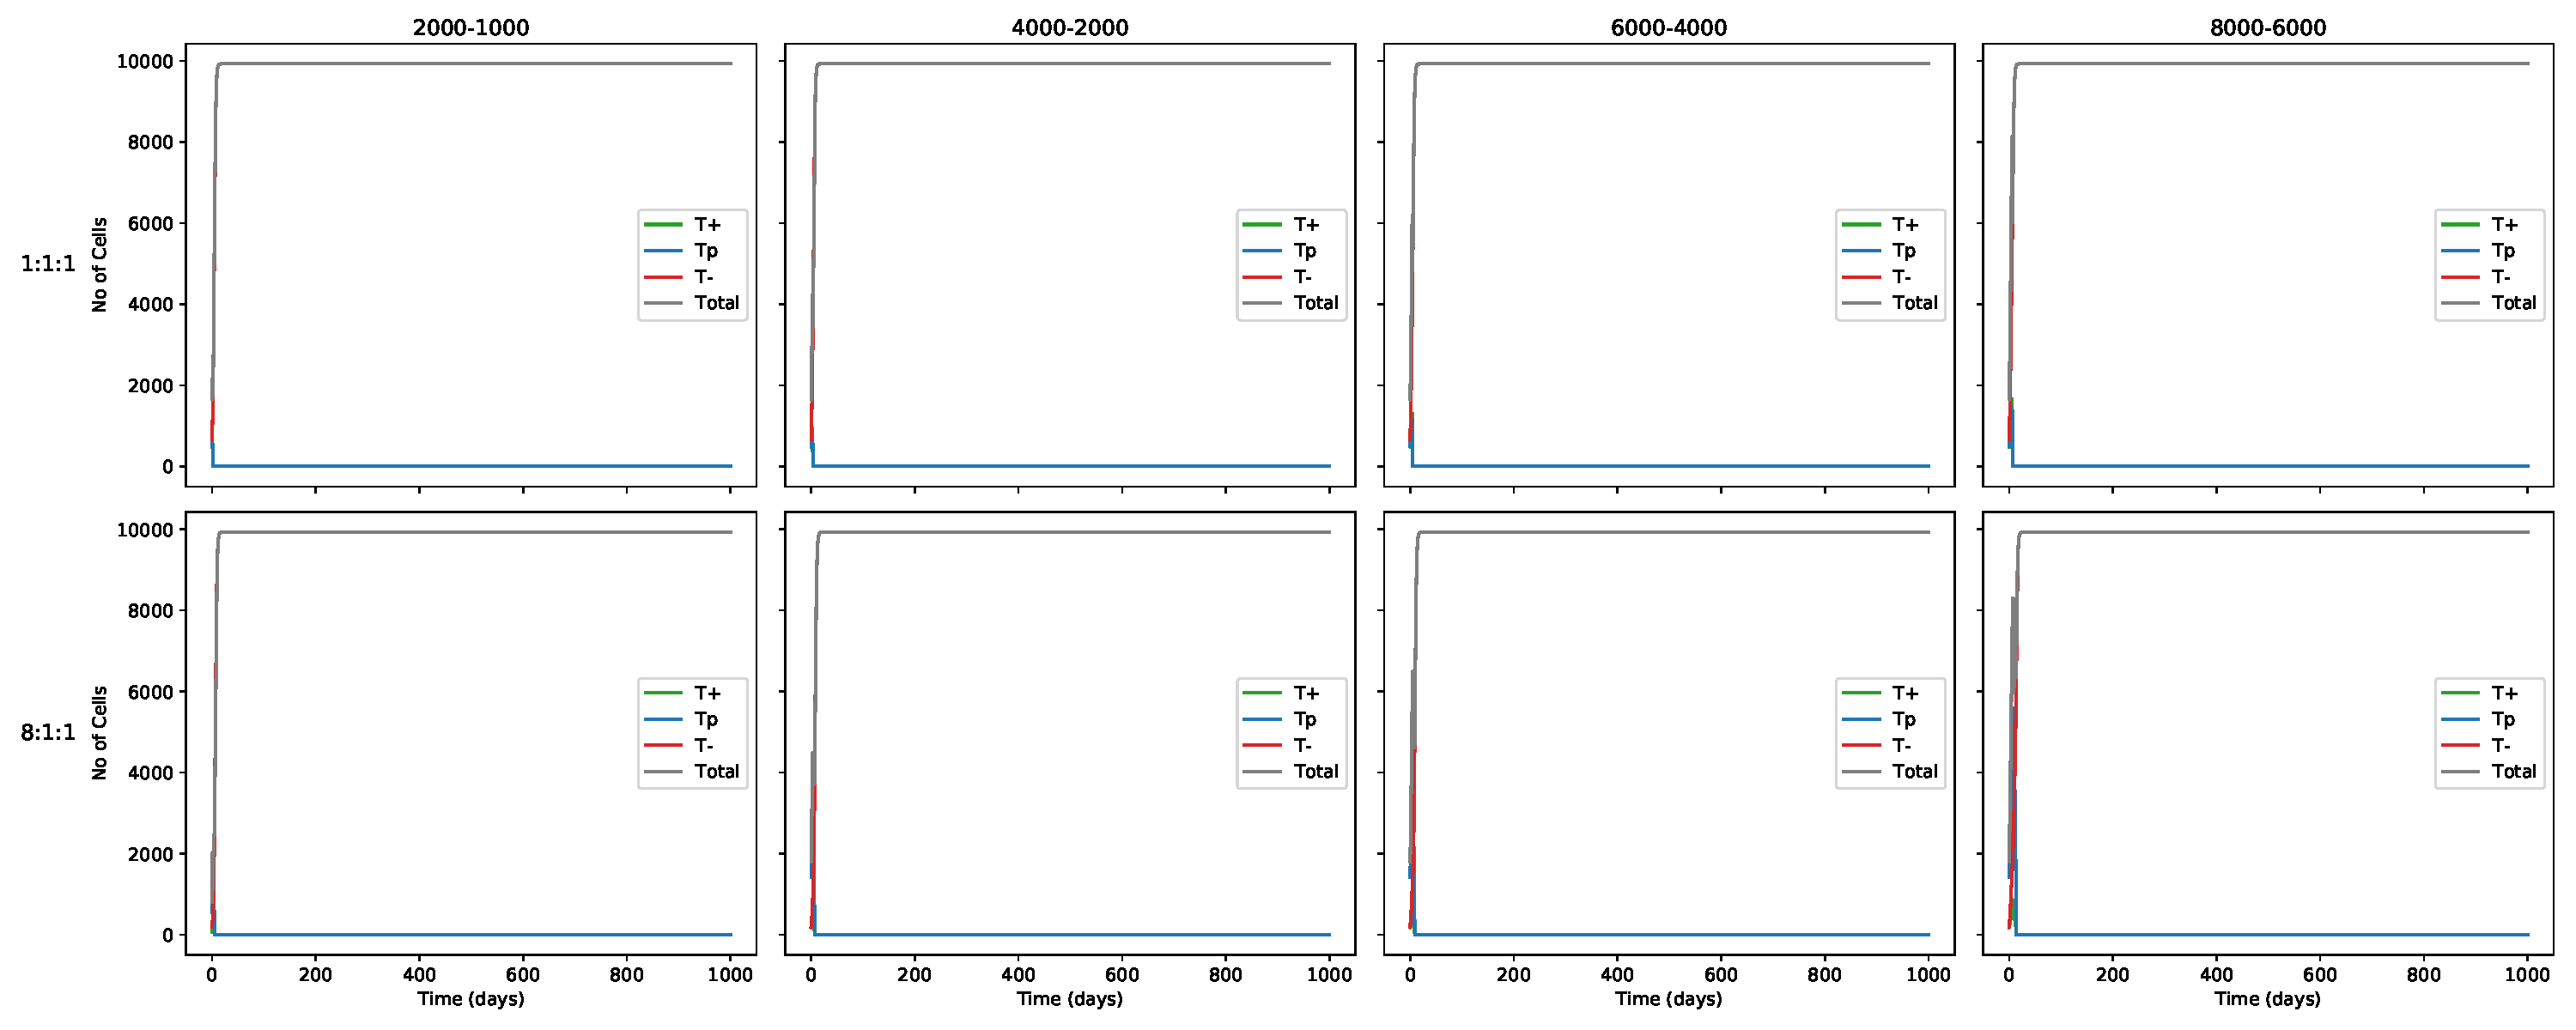
\includegraphics[width=\textwidth]{figures/All3_therapy-standardization-total}
  \end{subfigure}
  \begin{subfigure}[b]{\textwidth}
    \centering
    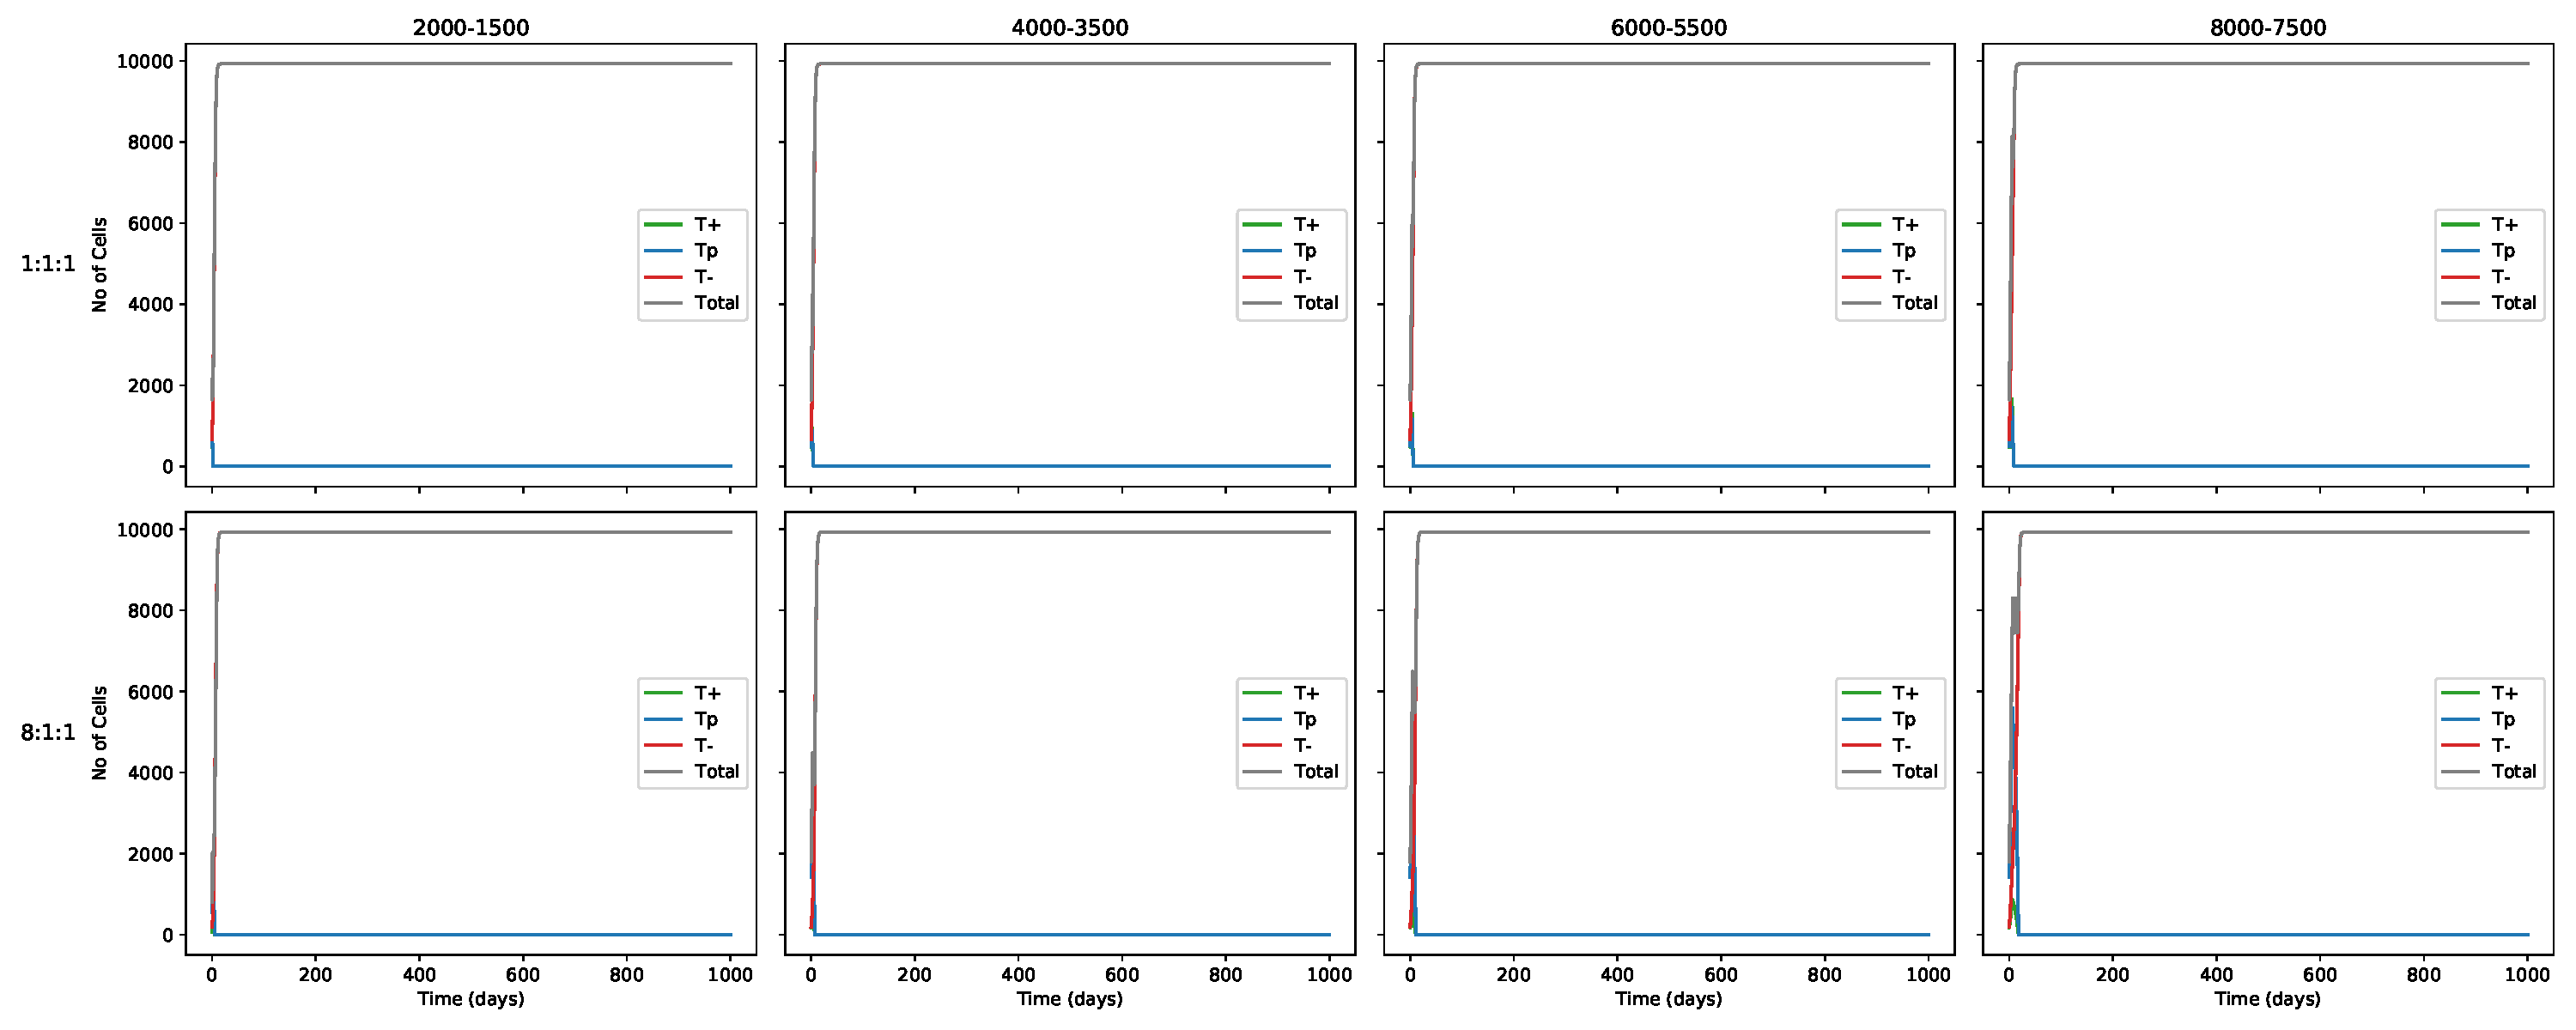
\includegraphics[width=\textwidth]{figures/All3_therapy-standardization-total-sw}
  \end{subfigure}
  \caption[Standardization of threshold conisdering all 3 cells for adaptive therapy]{Standardization of threshold considering all three cells for adaptive therapy, Columns: On-Off threshold, Rows: $T^p:T^+:T^-$ Seeding}
  \label{fig_therapy-AT_standardization-Total}
\end{figure}
